\documentclass[11pt]{article}

\usepackage[a4paper,margin=29mm]{geometry}
\usepackage[T1]{fontenc}
\usepackage{lmodern}
\usepackage{microtype}
\usepackage{amsmath,amssymb,amsthm,mathtools,mathrsfs}
\usepackage{array,booktabs}
\usepackage{enumitem}
\usepackage{needspace}
\usepackage{tikz}
\usetikzlibrary{arrows.meta,positioning}
\usepackage[hidelinks]{hyperref}

\newtheorem{theorem}{Theorem}[section]
\newtheorem{proposition}[theorem]{Proposition}
\newtheorem{lemma}[theorem]{Lemma}
\newtheorem{corollary}[theorem]{Corollary}
\theoremstyle{definition}
\newtheorem{definition}[theorem]{Definition}
\theoremstyle{remark}
\newtheorem{remark}[theorem]{Remark}

\newcommand{\F}{\mathbf F}
\newcommand{\Q}{\mathbf Q}
\newcommand{\Z}{\mathbf Z}
\newcommand{\PP}{\mathbf P}
\newcommand{\Sym}{\operatorname{Sym}}
\newcommand{\Sing}{\operatorname{Sing}}
\newcommand{\Stab}{\operatorname{Stab}}
\newcommand{\PGL}{\operatorname{PGL}}
\newcommand{\Aug}{\operatorname{Aug}}
\newcommand{\End}{\operatorname{End}}
\newcommand{\Hom}{\operatorname{Hom}}
\newcommand{\Ext}{\operatorname{Ext}}
\newcommand{\Gal}{\operatorname{Gal}}
\newcommand{\Aut}{\operatorname{Aut}}
\newcommand{\cC}{\mathscr C}
\newcommand{\cG}{\mathscr G}

\title{The Golden Companion Correspondence}
\author{Tavis Rudd}
\date{August 2026}

\begin{document}
\begingroup
\makeatletter
\let\clebschmaintitle\@title
\def\@title{\large\textsc{Clebsch: Rigidity from Sparse Shadows --- }\textbf{V}\\[0.7em]
  \LARGE\clebschmaintitle}
\makeatother
\maketitle
\endgroup

\begin{center}
\small\itshape
From deep holes, a cubic takes shape; its companion finds its bearings,\\
the carrier stands fixed while their shadows move; from minimum words, the plane returns,\\
and \textbf{the scattered shadows gather home}.
\end{center}

\begin{abstract}
On the quadratic augmentation module of the six Sylow-\(5\) subgroups of
\(A_5\), we classify the normalized chordal and conference shadows that occur
in the Clebsch reconstruction series.  A chordal cubic first recovers a split
twelve-point \(C_5\)-orbit on its singular rational normal quartic.  The
stabilizer quotient of that orbit recovers the six-set, and the literal outer
permutation of the six-set recovers the oriented conference companion by a
single difference operator.  This gives an equivalence of the selected-line
chordal and conference groupoids.  Without the selected chordal line the map
is a residual double cover, not an equivalence; we compute the complete
marking dependency and its Klein-four sharpness action.

The classification places the signed cubic of Paper~II in one of the two
chordal lines of the \(A_5\)-invariant cubic pencil and returns the retained
outputs of Papers~I--III exactly.  We then extract the integral structure
forced by the recovered six-set.  The rank-five augmentation lattice and the
rank-six \(D\)-type lattice meet in the same four-dimensional binary heart.
More generally, a symmetric conference operator of order
\(n\equiv2\pmod4\) minimally stabilizes \(D_n^\vee\), with a split/inert
mod-eight residue dichotomy.  At \(n=6\), normalization before reduction
produces the unique nonsplit extension of a trivial \(\F_4\)-line by the
natural \(\F_4A_5\)-module.  Golden reversal becomes Frobenius on this heart.
Thus the residual involution in the geometric correspondence and the
residual involution in the integral normalization are the same marked
symmetry.
\end{abstract}

\noindent\textbf{Keywords.} chordal cubic; conference matrix; reconstruction;
root lattice; modular representation; Frobenius descent.

\smallskip
\noindent\textbf{2020 Mathematics Subject Classification.} 20C20, 05B20,
14N15, 11H06.

\section{Introduction and statement}
\label{sec:introduction}

An invariant can retain the correct symmetry and still be the wrong
invariant.  The irreducible five-dimensional representation of \(A_5\) has a
two-dimensional space of invariant cubics.  One line contains the triangle
cubic of an oriented conference matrix.  Two other points of the pencil are
chordal cubics, each singular along a rational normal quartic.  The signed
matching tensor of Paper~II lands on a chordal line, not on the conference
line.  The purpose of this paper is to explain why that failure is exactly
what makes the reconstruction work.

The explanation has four steps.  First, the singular quartic of a chordal
cubic contains a distinguished split \(A_5/C_5\)-orbit.  Sending each point
to its stabilizer produces the canonical quotient
\[
              A_5/C_5\longrightarrow A_5/D_{10},
\]
and hence recovers the six-axis carrier.  Second, the nontrivial outer
permutation of this six-set acts linearly on the invariant pencil.  Its
difference from the identity carries either selected chordal line
isomorphically onto the conference line.  Third, retaining the standard
quadratic form on the augmentation removes the scalar inertia that a cubic
alone would leave after field extension.  The resulting categories are
therefore honest metric groupoids, and their exact forgetful fibres can be
computed.  Fourth, the same recovered six-set supports an integral
root--weight normalization.  In order six, its residue is the natural
\(\F_4A_5\)-heart, and outer reversal acts on it by Frobenius.

The exceptional six-point dictionaries and Joubert--Segre constructions are
classical; we use Howard--Millson--Snowden--Vakil
\cite[\S\S1.1--1.6 and 2.1--2.4]{HMSVOuter}.  The invariant pencil and its
chordal members are due, in the form needed here, to Pinardin--Zhang
\cite[\S6.2]{PinardinZhang2025}; the unmarked chordal geometry has the larger
automorphism group \(\PGL_2\) \cite[\S5]{CheltsovEtAl2025Chordal}.
Conference switching follows Goethals--Seidel
\cite[\S\S1--3]{GoethalsSeidel1967}, and the order-six switching class is
classical \cite{BMS1979}.  Our claims concern the marked compatibility,
normalization, exact information loss, and the root--weight residue obtained
when these ingredients are composed.  We make no priority claim beyond this
attribution boundary.

\Needspace{18\baselineskip}
\medskip
\noindent\textbf{Series perspective.}
\emph{Clebsch: Rigidity from Sparse Shadows} asks when incomplete invariants
determine the structures that produced them.  Papers~I and III reconstruct
marked conference companions, whereas Paper~II reconstructs a signed chordal
companion.  The present paper proves that these are exact marked forms of one
carrier and computes the ambiguity left by forgetting their markings.
Paper~IV is a parallel lower branch: its minimum words reconstruct a conic
plane and an \(\F_8\)-operator field.  The two branches have no common geometric
carrier, but their final residual markings are instances of the same
Frobenius-orbit principle.  Figure~\ref{fig:series-map} records this division.

\begin{figure}[ht]
\centering
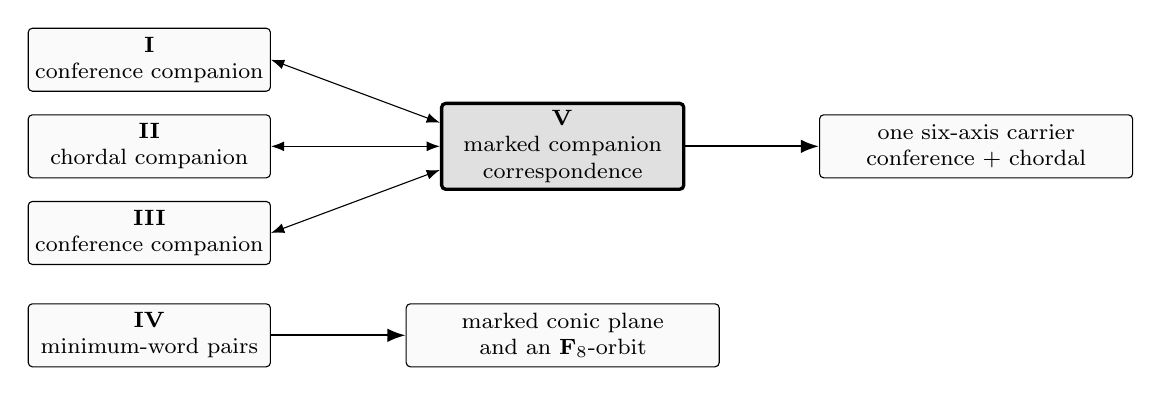
\begin{tikzpicture}[
  x=1cm,y=1cm,>=Latex,
  paper/.style={draw,rounded corners=1.5pt,fill=black!2,
    align=center,font=\footnotesize,minimum height=8mm,text width=29mm,
    inner sep=2.5pt},
  active/.style={paper,very thick,fill=black!12},
  package/.style={paper,text width=38mm}
]
\node[paper]   (p1) at (0,1.45) {\textbf{I}\\conference companion};
\node[paper]   (p2) at (0,0.35) {\textbf{II}\\chordal companion};
\node[paper]   (p3) at (0,-0.75) {\textbf{III}\\conference companion};
\node[active]  (p5) at (5.25,0.35) {\textbf{V}\\marked companion correspondence};
\node[package] (gold) at (10.5,0.35) {one six-axis carrier\\conference \(+\) chordal};
\node[paper]   (p4) at (0,-2.05) {\textbf{IV}\\minimum-word pairs};
\node[package] (plane) at (5.25,-2.05) {marked conic plane\\and an \(\F_8\)-orbit};
\draw[<->] (p1.east) -- ([yshift=3mm]p5.west);
\draw[<->] (p2.east) -- (p5.west);
\draw[<->] (p3.east) -- ([yshift=-3mm]p5.west);
\draw[->,thick] (p5.east) -- (gold.west);
\draw[->,thick] (p4.east) -- (plane.west);
\end{tikzpicture}
\caption{Series map.  Upper double arrows are the exact marked transports and
returns proved here; the right arrow is the common-carrier theorem.  The
lower solid arrow is Paper~IV's independent reconstruction.  Only their
residual Frobenius-orbit profiles are compared.}
\label{fig:series-map}
\end{figure}

Put \(k=\F_{11}\), \(G=A_5\), and let

\[
 \Omega_0=\operatorname{Syl}_5(G),\qquad
 A_0=\Aug(k^{\Omega_0}),\qquad
 Q_0(x)=\sum_{\omega\in\Omega_0}x_\omega^2.
\]

Thus \(|\Omega_0|=6\), \(A_0\) has dimension five, and in the basis
\(e_i-e_6\) the Gram matrix of \(Q_0\) is \(I+J\), of determinant \(6\).
Write

\[
                   \Pi=\Sym^3(A_0^*)^G.
\]

The standard order-six conference class determines an unordered pair of
opposite actual cubics \(\{\pm c_B\}\subset\Pi\).  A literal outer permutation
of \(\Omega_0\) induces a linear involution \(q_\Pi\) on \(\Pi\); its definition
is independent of the chosen representative of the outer coset because \(G\)
acts trivially on \(\Pi\).

\begin{definition}[Metric chordal shadow]
\label{def:metric-chordal-shadow}
Let \(K/k\) be a field extension.  A metric chordal shadow over \(K\) is the
neutral scalar extension of \((A_0,Q_0)\), together with a nonzero actual
cubic \(h\in\Pi_K\) whose saturated Jacobian scheme is a rational normal
quartic.  If

\[
                   (q_\Pi-1)h=\alpha c_B,
\]

for one of the coefficient-normalized conference generators, the shadow is
\emph{normalized} when \(\alpha^2=8^2\).  Morphisms are \(G\)-equivariant
\(Q_0\)-isometries preserving the stated actual generators and exactly the
coordinated relabelings explicitly allowed in the source package.
\end{definition}

The word \emph{neutral} is deliberate.  We classify scalar extensions of this
fixed quadratic carrier, not arbitrary twisted \(K\)-forms.  The quadratic
form is also essential: over a field containing \(\mu_3\), a scalar
\(\zeta I\) with \(\zeta^3=1\) fixes every cubic; preservation of \(Q_0\)
adds \(\zeta^2=1\), and hence forces \(\zeta=1\).

Our main result is most compactly stated as follows.  The groupoids named in
the theorem are defined independently in Section~\ref{sec:groupoids}.

\begin{theorem}[Intrinsic companion classification]
\label{thm:intrinsic-companion-classification}
For every extension \(K/k\), neutral scalar extension gives natural
equivalences

\[
 \cC_{\mathrm{conf}}^{L}(K)
   \simeq \cG_{\mathrm{met}}(K)
   \simeq \cC_{\mathrm{ch}}(K).
\]

Here the first groupoid consists of oriented order-six conference packages
with a selected compatible chordal line, the second of the derived expanded
metric carriers, and the third of normalized metric chordal shadows.  Under
these equivalences:

\begin{enumerate}[label=\textup{(\roman*)},leftmargin=2.4em]
\item the singular quartic recovers a split degree-twelve scheme \(Z_5\) and
  a canonical stabilizer quotient \(Z_5\to\Omega_0\);
\item the oriented conference generator is

  \[
                        c=8^{-1}(q_\Pi-1)h;
  \]
\item the selected-line functors return all retained source data of
  Papers~I--III, but no source-local chart or global cover not included in the
  bridge datum;
\item after the selected chordal line is forgotten,

  \[
     \cC_{\mathrm{conf}}(K)
       \simeq \cC_{\mathrm{ch}}(K)/\langle uq\rangle,
  \]
  where \(u=-I\) and \(uq:(L,h,c)\mapsto(qL,-qh,c)\).  Thus the unselected
  map is a residual \(C_2\)-torsor, not an equivalence.
\end{enumerate}
\end{theorem}

\begin{theorem}[Normalization--residue theorem]
\label{thm:normalization-residue-intro}
The recovered six-set canonically distinguishes the rank-five augmentation
lattice from the rank-six \(D\)-type lattice, while identifying their common
binary heart.  For every normalized symmetric conference matrix \(B\) of
order \(n\equiv2\pmod4\), the operator

\[
                         \varphi_B=\frac{I+B}{2}
\]

minimally stabilizes \(D_n^\vee\), and

\[
       \varphi_B^2-\varphi_B=\frac{n-2}{4}I.
\]

Modulo two its coefficient algebra is \(\F_4\) when \(n\equiv6\pmod8\) and
\(\F_2\times\F_2\) when \(n\equiv2\pmod8\).  At \(n=6\), writing
\(M=D_6^\vee/2D_6^\vee\), there is a canonical nonsplit sequence

\[
 0\longrightarrow H\longrightarrow M\longrightarrow\F_4\longrightarrow0,
\]

where \(H\) is a natural two-dimensional \(\F_4A_5\)-module and

\[
       \Ext^1_{\F_4A_5}(\F_4,H)\cong\F_4.
\]

On the endomorphism field
\[
                         \End_{A_5}(H)=\F_4,
\]
golden reversal \(B\mapsto-B\) and the outer normalizer both restrict to
Frobenius.  Relative to the recovered six-set, the golden-orientation torsor
and the exotic Frobenius torsor are therefore the same principal
\(C_2\)-torsor.
\end{theorem}

Fix now the Paper-II \(H_3\) matching
\[
 M=\{01,25,37,49,68,10\,11\}
\]
on the twelve points of \(\PP^1(\F_{11})\).  Its stabilizer in
\(\operatorname{PSL}_2(11)\) is a group \(G\cong A_5\), acting transitively
on the six pairs of \(M\).  Write \(X_M\) for that six-set and
\[
 A_M=\bigl\{(u_x)_{x\in X_M}\in\F_{11}^{X_M}:
                 \textstyle\sum_xu_x=0\bigr\}
\]
for its augmentation module.  Paper~II constructs a ten-dimensional
quotient \(W\), an intrinsic pair of matching sheets, and their first
nonzero signed moment \(\mu_3\in\Sym^3(W)\)
\cite{RuddFactorization2026}.
Since the action on \(X_M\) is transitive, a pair stabilizer has order ten;
the order-ten subgroups of \(A_5\) are the self-normalizing groups
\(D_{10}\).  Thus \(X_M\cong A_5/D_{10}\).

Let \(W_5\) be the five-isotypic summand of \(W|_G\).  The invariant
self-duality of \(W_5\) turns the projection of \(\mu_3\) into a projective
cubic line \([H_M]\subset\PP(\Sym^3(W_5^*))\).

The retained Paper-II datum is the actual projected generator together with
its normalized multiplicity-one bridge to \((A_0,Q_0)\).  The target metric is
the fixed \(Q_0\); no isomorphism class of arbitrary quadratic forms is being
classified.  Section~\ref{sec:placement} proves that the image is one of the
normalized metric chordal shadows in Theorem
\ref{thm:intrinsic-companion-classification}.

\medskip
\noindent\textbf{Proof and reading map.}
\begin{center}
\footnotesize
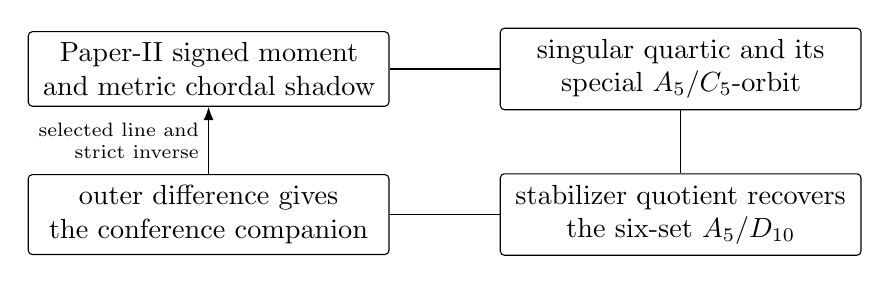
\begin{tikzpicture}[
  >=Latex,node distance=8mm and 14mm,
  box/.style={draw,rounded corners=1.5pt,align=center,text width=43mm,
    inner sep=4pt}, every edge/.style={draw,->}]
\node[box] (moment) {Paper-II signed moment\\and metric chordal shadow};
\node[box,right=of moment] (curve) {singular quartic and its\\special \(A_5/C_5\)-orbit};
\node[box,below=of curve] (axes) {stabilizer quotient recovers\\the six-set \(A_5/D_{10}\)};
\node[box,left=of axes] (conf) {outer difference gives\\the conference companion};
\draw (moment) -- (curve);
\draw (curve) -- (axes);
\draw (axes) -- (conf);
\draw[->] (conf) -- node[left,font=\scriptsize,align=right]
  {selected line and\\strict inverse} (moment);
\end{tikzpicture}
\end{center}

Section~\ref{sec:placement} gives the one Paper-II placement calculation.
Sections~\ref{sec:singular} and \ref{sec:outer-companion} prove the special
orbit and outer-difference bridge.  Section~\ref{sec:groupoids} upgrades the
round trip to an intrinsic classification and computes its marking fibres.
Section~\ref{sec:source-return} records the source-specific returns.
Sections~\ref{sec:lattice-tower}--\ref{sec:golden-residue} prove the integral
normalization--residue theorem.  Section~\ref{sec:residual-markings} compares
its \(C_2\)-rigidification with Paper~IV's separate \(C_3\)-rigidification.

\medskip
\noindent\textbf{Scope.}
The classification is intrinsic after the literal quadratic augmentation
carrier has been fixed.  It does not classify twisted forms of that carrier,
identify the chordal and conference cubics, or reconstruct source-local charts
that were not retained as bridge data.  The integral theorem likewise
identifies a common binary heart, not the two integral lattices themselves.
These distinctions are the information-loss content of the result rather than
technical qualifications.

\section{The metric chordal normal form}
\label{sec:placement}

The restriction of Paper II's quotient to \(G\) has character
\[
\begin{array}{c@{\qquad}ccccc}
\text{class}&1&2&3&5A&5B\\
\text{class size}&1&15&20&12&12\\
\chi_W&10&2&1&0&0
\end{array}
\]
and hence
\[
 W|_G\cong\mathbf1\oplus V_4\oplus V_5.
\]
The quotient and signed moment are imported from Paper~II's stable results
\emph{The \(3,6,10\) quotient ranks} and
\emph{Balanced sheets and cubic-first orientation}
\cite{RuddFactorization2026}; the displayed restriction is the character
calculation used here.  The field \(\F_{11}\) contains the fifth roots of
unity and \(\sqrt5=4\), and \(11\nmid60\), so it is a splitting field for
this calculation and the summands are absolutely irreducible.
Because \(11\nmid60\), the central character idempotent
\[
 e_5=\frac5{60}\sum_{g\in G}\chi_5(g)g
\]
is defined over \(\F_{11}\), is idempotent, and has rank five.  The
degree-six permutation character is \(\mathbf1+\chi_5\), so \(A_M\cong V_5\).
Schur's lemma gives
\[
 \dim_{\F_{11}}\operatorname{Hom}_G(A_M,e_5W)=1.
\]

\begin{proposition}[Paper-II placement]
\label{prop:paper-ii-placement}
After the outer-twisted multiplicity-one identification with \(A_0\), the
chosen-sheet projection of Paper~II's signed moment is a normalized metric
chordal shadow.  In standard binary-quartic coordinates it is
\[
 H=z_0z_2z_4+2z_1z_2z_3-z_0z_3^2-z_1^2z_4-z_2^3
   =\det\!\begin{pmatrix}
       z_0&z_1&z_2\\ z_1&z_2&z_3\\ z_2&z_3&z_4
     \end{pmatrix}.
\]
Its sheet reversal is \(-H\).  In the normalization used below, the
Paper-II pivot is \(3\), and the outer-difference coefficient is \(8\).
\end{proposition}

\begin{proof}
The representation-theoretic reduction is the calculation above.  Both
\(A_M\) and \(e_5W\) are copies of the absolutely irreducible module \(V_5\),
so their bridge is unique up to scalar.  There are two comparisons with the
binary-quartic model: the direct identification and its outer twist.  The
geometric discriminator is whether the Veronese quartic becomes the singular
curve.  The direct comparison fails this test and the outer-twisted
comparison passes it.

For completeness, we print the normalization leaf.  Choose the axis basis
\(e_i-e_6\) of \(A_M\) and Paper~II's reduced-pivot basis of \(W_5\).  The
bridge line is generated by
\[
 T=\begin{pmatrix}
 2&9&7&6&4\\
 0&9&10&10&6\\
 5&1&9&3&0\\
 0&3&10&1&6\\
 1&0&0&0&0
 \end{pmatrix}.
\]
The two generator relations of \(G\) verify
\(\rho_{W_5}(g)T=T\rho_{A_M}(g)\), and \(\det T\ne0\).  Put \(B_0=I+J\),
the Gram matrix of \(Q_0\).  If \(\nu\in\Sym^3(W_5)\) is the chosen-sheet
projection of \(\mu_3\), its axis cubic is
\[
 \widetilde h_M=
 \operatorname{Pol}\!\left(\Sym^3(B_0T^{-1})\nu\right).
\]
Its first nonzero coefficient is \(3\), so set
\(h_M=3^{-1}\widetilde h_M\).  The scalar is fixed before the sheet is
reversed.  Hence the other sheet is \(-h_M\), rather than a separately
projectivized generator.

After the nontrivial element of \(\operatorname{Out}(A_5)\), the unique
binary-quartic projectivity is
\[
 U=\begin{pmatrix}
 0&0&3&5&3\\
 4&1&1&10&4\\
 3&6&3&0&0\\
 5&1&6&10&5\\
 9&10&10&7&1
 \end{pmatrix}.
\]
With the pullback convention \(U(h)(z)=h(Uz)\), substitution of
\[
                 [s:t]\longmapsto[s^4:s^3t:s^2t^2:st^3:t^4]
\]
in the five first derivatives of \(U(h_M)\) gives zero.  A cubic singular
along a rational normal quartic is its secant, hence is a scalar multiple of
the Hankel determinant.  Comparing the coefficient of \(z_0z_2z_4\) gives
the scalar \(8\), so \(U(h_M)=8H\).  The conference cubic has six isolated
nodes by Paper~I and therefore spans a different line.  This proves the
placement without an exhaustive cubic comparison.
\end{proof}

The displayed matrices only fix the bridge between the frozen Paper-II basis
and the intrinsic carrier.  Every subsequent argument uses the recovered
metric shadow, its special orbit, and its normalizer.  The exact replay named
in Section~\ref{sec:verification} checks this normalization leaf
independently, but no later theorem depends on a coefficient census.

\section{The singular quartic recovers the axes}
\label{sec:singular}

\begin{lemma}[Singular locus of the Hankel determinant]
\label{lem:hankel-singular-locus}
Over \(\F_{11}\), the singular scheme of \(H=0\) is the rational normal
quartic \(R\).
\end{lemma}

\begin{proof}
The five partial derivatives are
\[
\begin{split}
 z_2z_4-z_3^2,&\qquad 2(z_2z_3-z_1z_4),\\
 z_0z_4+2z_1z_3-3z_2^2,&\qquad 2(z_1z_2-z_0z_3),\\
 z_0z_2-z_1^2.&
\end{split}
\]
Let \(I_R\) be the ideal of the six \(2\)-by-\(2\) minors of
\[
 \begin{pmatrix}z_0&z_1&z_2&z_3\\z_1&z_2&z_3&z_4\end{pmatrix}.
\]
These minors define the rational normal quartic scheme.  Four are scalar
multiples of the first, second, fourth, and fifth displayed derivatives.
Write the other two as
\[
 A=z_0z_4-z_1z_3,\qquad B=z_1z_3-z_2^2.
\]
The middle derivative is \(A+3B\), so the Jacobian ideal \(J\) is contained
in \(I_R\).  Conversely, on \(D(z_2)\), the identity
\[
 z_2A=z_0(z_2z_4-z_3^2)+z_3(z_0z_3-z_1z_2)
\]
puts \(A\), and then \(B\), in \(J_{z_2}\).  On \(D(z_0)\),
\[
 z_0B=z_1(z_0z_3-z_1z_2)-z_2(z_0z_2-z_1^2)
\]
does the same; the symmetric identity handles \(D(z_4)\).  These three
opens cover the projective Jacobian scheme, since \(z_0=z_2=z_4=0\) and the
outer two derivatives force \(z_1=z_3=0\).  Hence the saturated Jacobian
ideal equals \(I_R\), proving the scheme-theoretic assertion.
\end{proof}

\begin{proposition}[The special orbit and its stabilizer quotient]
\label{prop:special-orbit}
Let \(R\) be the singular quartic of a metric chordal shadow.  The scheme
\[
 Z_5=\coprod_{P\in\operatorname{Syl}_5(G)}R^P
\]
is split finite étale of degree twelve.  Every geometric point has exact
stabilizer \(C_5\), and the stabilizer map is the canonical double cover
\[
                 Z_5\longrightarrow\Omega_0.
\]
For the Paper-II shadow this quotient is the original six-set \(X_M\).
\end{proposition}

\begin{proof}
The rational normal quartic spans \(\PP(A_0)\), so an element acting trivially
on \(R\) acts projectively trivially on \(A_0\).  The augmentation action is
faithful, and therefore \(G\) acts faithfully on \(R\cong\PP^1\), hence through
\(\PGL_2(11)\).  Its composite with the determinant-class quotient
\(\PGL_2(11)/\operatorname{PSL}_2(11)\cong C_2\) is trivial because
\(G\cong A_5\) is simple.  Thus \(G\) lies in
\(\operatorname{PSL}_2(11)\).  For \(x\in R(\F_{11})\), its
stabilizer lies in the
order-\(55\) Borel subgroup of \(\operatorname{PSL}_2(11)\), hence has order
dividing \(\gcd(60,55)=5\).  A Sylow \(5\)-subgroup is split and fixes two
points.  Distinct Sylow \(5\)-subgroups cannot share a fixed point, since
the point stabilizer has order at most five.  The six Sylow subgroups
therefore supply \(6\cdot2=12\) distinct points, exhausting \(R(\F_{11})\).
Every point stabilizer is \(C_5\), the action is transitive, and the six
fixed-point pairs form
\[
 G/N_G(C_5)\cong A_5/D_{10}.
\]
The stabilizer of each pair of the original matching is also \(D_{10}\), and
this subgroup is self-normalizing in \(G\).  Hence it fixes a unique matching
pair in the transitive \(G/D_{10}\) action.  Sending a singular point
to the matching pair fixed by the normalizer of its stabilizer therefore
gives the intrinsic map
\[
 A_5/C_5\longrightarrow A_5/D_{10},
 \qquad gC_5\longmapsto gN_G(C_5),
\]
with fibres of size two.  This proves the assertion over \(k\).

The fixed points of a generator of \(C_5\) are its two distinct eigenlines,
already defined over \(k\) because \(\mu_5\subset k^\times\).  Thus the six
pairs are reduced, disjoint, and constant.  The description commutes with
every scalar extension \(K/k\), proving the scheme statement.
\end{proof}

\begin{lemma}[The intrinsic conference pair]
\label{lem:unoriented-conference-companion}
The recovered \(G\)-set \(\Omega_0\cong A_5/D_{10}\) determines a unique
unordered pair \(\{[B],[-B]\}\) of \(G\)-invariant order-six conference
switching classes.  Coefficient normalization gives an unordered pair of
actual triangle cubics \(\{\pm c_B\}\subset\Pi\).
\end{lemma}

\begin{proof}
Normalize a symmetric conference signing by switching so that its first row
is positive.  Orthogonality with that row forces every other row to have two
positive and two negative entries away from the first coordinate and its
diagonal.  The negative entries therefore form a simple two-regular graph on
five vertices, hence a pentagon.  All pentagons are relabelled copies of one
another; complementing the pentagon gives the opposite switching class.
The natural six-point \(A_5\)-action preserves this class, and its two
orientations give opposite triangle cubics on the augmentation.  More
precisely, the automorphism group of an oriented order-six conference class
is the transitive \(A_5\).  Identify it with the recovered
\(G\leq S(\widehat X_M)\).  Two such identifications differ through
\[
 N_{S_6}(G)/G\cong C_2,
\]
and the nontrivial coset exchanges the class with its opposite.  Hence the
unordered opposite pair, and therefore its projective triangle-cubic line,
is intrinsic to the fixed recovered \(G\)-set.  This classical uniqueness
and pentagon representative also appear in
Bussemaker--Mathon--Seidel
\cite[pp.~12, 21, and Table~9 on p.~83]{BMS1979}; our switching
convention follows Goethals--Seidel \cite[\S\S1--3]{GoethalsSeidel1967}.
\end{proof}

Paper~I's corollary \emph{Nodes, symmetry, and integral commutant} proves
that this triangle cubic has exactly six ordinary nodes in projective-frame
position \cite{RuddRigidity2026}.  Since \(H_M\) is singular along a curve,
the conference and chordal lines are distinct.  The point is causal: the
conference pair was constructed from the recovered six-set, not inserted
among the recognition axioms.

\section{Outer difference and the oriented companion}
\label{sec:outer-companion}

The ordinary character of the augmentation module is
\[
                    \chi_5=(5,1,-1,0,0)
\]
on the classes \(1,2A,3A,5A,5B\).  The symmetric-cube formula gives
\[
       \chi_{\Sym^3 A_0^*}=(35,3,2,0,0),
\]
and therefore
\[
 \dim\Pi=\frac{35+15\cdot3+20\cdot2}{60}=2.
\]
Maschke's theorem and the Reynolds idempotent show that this calculation
commutes with every extension \(K/k\).

The construction of the outer operator is linear, not merely projective.
Let \(\tau\) be an involutive permutation in the nontrivial coset of
\(N_{S(\Omega_0)}(G)/G\), and let \(P_\tau\) act on the literal augmentation
\(A_0\).  If an abstract copy \(A\) of the five-dimensional module is in use
and \(T:A\to A_0\) is any nonzero intertwiner, put
\[
                         q=T^{-1}P_\tau T.
\]
Changing the scalar of \(T\) changes nothing.  Changing \(\tau\) by an
element of \(G\) changes nothing on \(\Pi\).  Thus the induced
\(q_\Pi\in\operatorname{GL}(\Pi)\) is canonical relative to the recovered
six-set.

\begin{proposition}[Normalized outer action]
\label{prop:outer-pencil-action}
Let \(c_B\) be either coefficient-normalized conference generator and let
\(h\) be the corresponding normalized Paper-II chordal generator.  In the
ordered basis \((c_B,h)\),
\[
              [q_\Pi]=\begin{pmatrix}-1&8\\0&1\end{pmatrix}.
\]
Consequently the conference line is \(\Pi^-=\ker(q_\Pi+1)\), the two chordal
lines are exchanged, and
\[
          (q_\Pi-1)h=8c_B.
\]
\end{proposition}

\begin{proof}
Take the literal odd permutation \((3\ 4\ 5\ 6)\) of the recovered six-set.
In the basis \(e_i-e_6\), its augmentation matrix is
\[
 Q=\begin{pmatrix}
 1&0&0&0&0\\
 0&1&0&0&0\\
 -1&-1&-1&-1&-1\\
 0&0&1&0&0\\
 0&0&0&1&0
 \end{pmatrix}.
\]
Reversing the conference class changes every triangle sign, hence sends
\(c_B\) to \(-c_B\).  Proposition~\ref{prop:paper-ii-placement} identifies
the Paper-II line with the chordal line and fixes its scalar.  Comparing one
coefficient in \(q_\Pi h-h\) with the same coefficient of \(c_B\) gives
\(8\).  Since both sides lie in the one-dimensional anti-invariant line,
this single comparison proves the displayed formula.  The independence of
the outer representative was proved above.
\end{proof}

\begin{corollary}[Selected-line bridge]
\label{cor:selected-line-bridge}
For either chordal line \(L\subset\Pi\), the restriction
\[
 q_\Pi-1:L\longrightarrow\Pi^-
\]
is an isomorphism.  On the punctured lines it is \(K^\times\)-equivariant.
On normalized generators its forward and inverse maps are
\[
 h\longmapsto c=8^{-1}(q_\Pi-1)h,\qquad
 c\longmapsto h=((q_\Pi-1)|_L)^{-1}(8c).
\]
They carry \(-h\) to \(-c\).
\end{corollary}

\begin{proof}
The assertion on the Paper-II line is Proposition
\ref{prop:outer-pencil-action}.  The other chordal line is \(q_\Pi L\), and
\(q_\Pi^2=1\), so the restriction there is nonzero as well.  Every remaining
assertion follows from linearity.
\end{proof}

The line \(L\) is not cosmetic.  The conference package remembers the
unordered pair \(\{L,q_\Pi L\}\), but no one member of it.  Moreover
\[
       (q_\Pi-1)(-q_\Pi h)=(q_\Pi-1)h.
\]
Thus \(h\) and \(-q_\Pi h\) have the same oriented conference companion.
This residual involution is the precise obstruction to an unselected
equivalence.

\section{Intrinsic groupoids and exact marking fibres}
\label{sec:groupoids}

We now define the classification categories without referring to the image
of a reconstruction functor.

\begin{definition}[The three companion groupoids]
\label{def:three-groupoids}
For an extension \(K/k\), let:
\begin{enumerate}[label=\textup{(\alph*)},leftmargin=2.4em]
\item \(\cC_{\mathrm{ch}}^\times(K)\) be the groupoid of neutral metric
  chordal shadows with arbitrary nonzero actual generator, and let
  \(\cC_{\mathrm{ch}}(K)\) be its full normalized subgroupoid
  \(\alpha^2=8^2\);
\item \(\cG_{\mathrm{met}}(K)\) be the groupoid of tuples derived from such a
  normalized shadow:
  \[
  (A_0,Q_0,\Pi,R_h,Z_5,\Omega_0,q_\Pi,L,h,c,[B]);
  \]
  every entry after \(h\) is required to be the construction of
  Sections~\ref{sec:singular} and \ref{sec:outer-companion}, not an
  independent recognition axiom;
\item \(\cC_{\mathrm{conf}}^L(K)\) be the groupoid of oriented order-six
  conference packages \((\Omega_0,[B],c)\), together with a selected chordal
  line \(L\subset\Pi_K\) for which
  \(((q_\Pi-1)|_L)^{-1}(8c)\) is a normalized metric chordal shadow.
\end{enumerate}
Morphisms are ambient \(G\)-equivariant \(Q_0\)-isometries, switching, and
the coordinated relabelings explicitly retained by the object.  Let
\(\cC_{\mathrm{conf}}(K)\) be obtained by forgetting \(L\).
\end{definition}

This definition does not assume the conclusions that make the construction
work.  In particular, the chordal locus, the special orbit, the conference
pair, and the scalar \(8\) were proved before the groupoids were introduced.

\begin{proposition}[Strict rigidity]
\label{prop:strict-rigidity}
The functors
\[
 \cC_{\mathrm{ch}}(K)\longrightarrow\cG_{\mathrm{met}}(K)
 \longleftarrow\cC_{\mathrm{conf}}^L(K)
\]
are fully faithful and essentially surjective.
\end{proposition}

\begin{proof}
Starting with a chordal shadow, Lemma
\ref{lem:hankel-singular-locus} and Proposition~\ref{prop:special-orbit}
recover \(R_h\), \(Z_5\), and \(\Omega_0\).  Lemma
\ref{lem:unoriented-conference-companion} recovers the conference pair, and
the literal normalizer recovers \(q_\Pi\).  Proposition
\ref{prop:outer-pencil-action} then identifies the normalized orientation
\[
                      c=8^{-1}(q_\Pi-1)h.
\]
This proves essential surjectivity from the chordal side.  Starting from the
selected-line conference package, Corollary~\ref{cor:selected-line-bridge}
recovers \(h\), after which the same construction returns every derived
entry.  This proves essential surjectivity from the conference side.

For full faithfulness, a projectivity is determined by its permutation of the
recovered six-node projective frame.  Two linear lifts of that projectivity
differ by a scalar \(\lambda\).  Preserving \(Q_0\) and the actual cubic gives
\(\lambda^2=\lambda^3=1\), hence \(\lambda=1\); this is where the metric
removes the hidden \(\mu_3\)-inertia.  Preservation of the frame,
\(q_\Pi\), and \(h\) then forces preservation of the special divisor, the
conference pair, and \(c\).  Conversely, every allowed coordinated
relabeling of the six-set induces one such isometry.  Hence both Hom maps are
bijective.
\end{proof}

Proposition~\ref{prop:strict-rigidity} proves the selected-line equivalences
in Theorem~\ref{thm:intrinsic-companion-classification}.  The unselected
statement follows from the actual involution
\[
                         uq:(L,h,c)\longmapsto(qL,-qh,c),
\]
which is fixed-point free and preserves the conference package.  Since
\[
                  (q_\Pi-1)(-q_\Pi h)=(q_\Pi-1)h,
\]
its two orbits are exactly the fibres of the forgetful functor.

\subsection{The dependency lattice}

The marking structure is not the Boolean lattice on a list of names.  Its
basic implications are
\[
 h\Rightarrow L=Kh,\qquad (q_\Pi,h)\Rightarrow c,\qquad
 c\Rightarrow\Sing(c)=\Omega_0.
\]
Before scalar normalization, forgetting a generator while retaining its line
has fibre \(K^\times\).  After \(\alpha^2=8^2\), it has the two sheet signs.
With \(u=-I\), the three nontrivial actions are
\[
\begin{aligned}
 u&:(L,h,c)\longmapsto(L,-h,-c),\\
 q&:(L,h,c)\longmapsto(qL,qh,-c),\\
 uq&:(L,h,c)\longmapsto(qL,-qh,c).
\end{aligned}
\]
Here \(u\) is an automorphism only after the actual sign has been forgotten,
and \(q\) is a morphism only when coordinated outer relabeling is allowed.
At the fully forgotten vertex, and only there, these transformations give a
free transitive Klein-four action.

\begin{center}
\small
\renewcommand{\arraystretch}{1.18}
\begin{tabular}{@{}p{0.30\textwidth}p{0.22\textwidth}p{0.34\textwidth}@{}}
\toprule
retained datum & forgetful fibre & sharpness action\\
\midrule
line \(L\), no scalar normalization & \(K^\times\) & scalar
  trivializations of \(L\)\\
line \(L\), normalized generator & \(C_2\) & \(u:(h,c)\mapsto(-h,-c)\)\\
oriented \(c\), no selected \(L\) & \(C_2\) & \(uq\)\\
unordered chordal and conference pairs & \(C_2\times C_2\) & \(u,q\)\\
\bottomrule
\end{tabular}
\end{center}

After \(L\) is fixed, sheet sign and conference orientation are not
independent: \(8^{-1}(q_\Pi-1)\) identifies them.  The table therefore
records a dependency lattice rather than four unrelated counts.

\section{The source functors and their return}
\label{sec:source-return}

We next state exactly what is returned to the earlier papers.  Paper~II's
bridge includes the normalized intertwiner \(T\) of
Section~\ref{sec:placement}; its pivot \(3^{-1}\) is transported, not
recomputed after relabeling.  Papers~I and III begin with a conference
signing and add the choice of \(L\).  Paper~III's chart lift, scale,
outer/Petersen labels, and cross-identification remain bridge data rather
than reconstructed outputs.

\begin{corollary}[Source-by-source marked return]
\label{cor:source-by-source-return}
Relative to the markings in the following table, each of Papers~I--III maps
to the normalized metric carrier and is recovered at exactly the stated
output level.
\begin{center}
\small
\renewcommand{\arraystretch}{1.15}
\begin{tabular}{@{}>{\centering\arraybackslash}p{0.07\textwidth}
  >{\raggedright\arraybackslash}p{0.32\textwidth}
  >{\raggedright\arraybackslash}p{0.20\textwidth}
  >{\raggedright\arraybackslash}p{0.31\textwidth}@{}}
\toprule
paper & retained source output & target decoration & inverse returns\\
\midrule
I & conference switching class, axis carrier, orientation, and selected
  chordal line \(L\) & the metric core & the same class, carrier,
  orientation, and \(L\), modulo switching and relabeling\\
II & five-isotypic projected tensor with chosen sheet sign, marked axes, and
  \(T\) & \(W_5,T\), and the fixed pivot & the same projected tensor, sheet
  sign, six-axis carrier, and \(T\)\\
III & relative conference source, selected \(L\), and full bridge datum &
  \(\mathfrak m_{\mathrm{III}}\) & the same retained source, orientation,
  \(L\), and bridge datum\\
\bottomrule
\end{tabular}
\end{center}
No inverse is asserted outside the declared retained output.
\end{corollary}

\begin{proof}
Paper~I's \emph{Support cubic and golden continuation} and its six-node
corollary recover the conference signing, orientation, and axis carrier
\cite{RuddRigidity2026}.  Paper~III's \emph{Relative marked orientation
bridge} supplies the same conference source relative to its fixed bridge
datum \cite{RuddPassages2026}.  Given \(L\), Corollary
\ref{cor:selected-line-bridge} recovers the unique normalized \(h\in L\).
Returning forgets this derived generator and leaves the source data
unchanged.

For Paper~II, \emph{Balanced sheets and cubic-first orientation} supplies
the signed generator.  Proposition~\ref{prop:special-orbit} recovers the
axis carrier, and Corollary~\ref{cor:selected-line-bridge} supplies \(c\).
Writing \(B_0=I+J\), the exact forward and reverse tensor maps are
\[
 h=3^{-1}\operatorname{Pol}\!\left(\Sym^3(B_0T^{-1})\nu\right),
 \qquad
 \nu=\Sym^3(TB_0^{-1})\operatorname{Pol}^{-1}(3h).
\]
Thus the pivot, polynomialization, self-duality, and bridge are undone in
the reverse order.  Every operation is induced by the marked axis
relabeling, so the return is natural.
\end{proof}

\begin{corollary}[Neutral base change]
\label{cor:stabilizer-stratified-base-change}
Every construction and equivalence above commutes with scalar extension
\(K/k\).  In particular,
\[
 Z_{5,K}=\coprod_{P\in\operatorname{Syl}_5(G)}R_K^P
       \longrightarrow \operatorname{Syl}_5(G)_K
\]
is the constant split double cover
\((G/C_5)_K\to(G/D_{10})_K\).
\end{corollary}

\begin{proof}
The Reynolds idempotent commutes with scalar extension, the Hankel Jacobian
identity is scheme-theoretic over \(k\), and the \(C_5\)-fixed eigenlines are
already split over \(k\).  The conference pair, the normalizer action, and
the forward and inverse tensor maps are defined over \(k\); the scalars \(3\)
and \(8\) remain units after extension.
\end{proof}

This is a theorem about neutral scalar extensions of the fixed carrier.  It
does not classify arbitrary twisted \(K\)-forms and does not create a new
matching problem on \(\PP^1(\F_{11^m})\).

\section{The two integral lattices of the six-set}
\label{sec:lattice-tower}

Let \(\Omega\) be any six-set and put \(P=\Z^\Omega\).  The reconstruction
produces two different integral lattices:
\[
 A_{\mathrm{aug}}(\Omega)=\ker(P\xrightarrow{\sum}\Z),
 \qquad
 D(\Omega)=\{x\in P:\textstyle\sum_\omega x_\omega\equiv0\pmod2\}.
\]
The first has rank five and is the integral source for the later symplectic
envelope in the series.  The second has rank six.  For the standard
permutation pairing,
\[
                  D(\Omega)^\vee=P+\Z\frac{\mathbf1_\Omega}{2}.
\]
Conflating the two lattices hides both the rank and the factor of two.

\begin{proposition}[The common six-point heart]
\label{prop:common-heart}
The two lattices canonically determine the same four-dimensional
\(\F_2S(\Omega)\)-module
\[
 H_\Omega=\Aug(\F_2^\Omega)/\langle\mathbf1_\Omega\rangle.
\]
More precisely, reduction of \(A_{\mathrm{aug}}(\Omega)\) is
\(\Aug(\F_2^\Omega)\), while
\[
 D(\Omega)/2P\cong\Aug(\F_2^\Omega);
\]
quotienting the common constant line gives \(H_\Omega\).
\end{proposition}

\begin{proof}
A binary vector of even coordinate sum lifts to an integral vector of sum
zero by changing one coordinate by an even integer.  This proves the first
surjectivity.  The definition of \(D(\Omega)\) proves the second
identification.  Since \(|\Omega|=6\) is even, the constant binary vector lies
in both reductions.  All maps are induced by the permutation lattice and
are therefore functorial in \(\Omega\).
\end{proof}

The rank-five and rank-six outputs meet at \(H_\Omega\); they do not become
the same lattice.  This is the entire integral interface exported by Paper~V.

\section{Conference saturation}
\label{sec:conference-saturation}

We now prove the uniform lattice statement behind the golden specialization.
The closest classical analogue is Chapman's construction for skew conference
matrices and imaginary quadratic orders \cite{Chapman2001}; the symmetric
spectral setting is discussed by Haemers--Parsaei Majd
\cite{HaemersParsaeiMajd2022}.  We need only the elementary real,
root--weight statement below.

\begin{theorem}[Symmetric-conference root--weight saturation]
\label{thm:conference-saturation}
Let \(B\) be a normalized symmetric conference matrix of order
\(n\equiv2\pmod4\), so \(B^2=(n-1)I\), and put
\[
 L=\Z^n,\qquad h=\frac{\mathbf1}{2},\qquad
 \varphi_B=\frac{I+B}{2}.
\]
Then \(D_n^\vee=L+\Z h\) is the minimal over-lattice of \(L\) stable under
\(\varphi_B\), independently of switching, and
\[
              \varphi_B^2-\varphi_B=\frac{n-2}{4}I.
\]
The coefficient algebra acting faithfully on \(D_n^\vee/2D_n^\vee\) is
\[
 \F_2[t]\big/\left(t^2+t+\frac{n-2}{4}\right).
\]
It is \(\F_4\) for \(n\equiv6\pmod8\) and
\(\F_2\times\F_2\) for \(n\equiv2\pmod8\).
\end{theorem}

\begin{proof}
Normalize the first row of \(B\) to be positive off the diagonal.  Every
column of \(I+B\) is odd, so \(\varphi_B L\subset L+\Z h\), while
\[
                         \varphi_Be_0=h.
\]
Thus every stable over-lattice containing \(L\) contains \(h\).  Orthogonality
with the first row gives row sums \(n-1,1,\ldots,1\), and therefore, with
\(m=(n-2)/4\),
\[
                         \varphi_Bh=h+me_0.
\]
This proves stability and minimality.  A diagonal switching matrix sends
\(h\) to \(h\) modulo \(L\), so the lattice is switching-independent.

The polynomial identity follows directly from \(B^2=(n-1)I\).  Reducing it
modulo two gives the displayed algebra.  When \(m\) is odd the polynomial is
\(t^2+t+1\), hence the algebra is \(\F_4\).  When \(m\) is even it is
\(t(t+1)\).  The action is not a scalar quotient: in the basis
\(h,e_1,\ldots,e_{n-1}\),
\[
 \bar e_0=\sum_{i>0}\bar e_i,\qquad
 \bar\varphi_B(\bar e_0)=\bar h,
\]
so \(\bar\varphi_B\) is neither zero nor the identity.  The split algebra
therefore acts faithfully.
\end{proof}

\section{The golden residue}
\label{sec:golden-residue}

Specialize Theorem~\ref{thm:conference-saturation} to the oriented
order-six conference operator recovered above.  Put
\[
 L^{\max}=D_6^\vee,\qquad \varphi=\frac{I+B}{2},\qquad
 M=L^{\max}/2L^{\max}.
\]
Then \(\varphi^2-\varphi-1=0\), so \(M\) is a three-dimensional vector space
over \(\F_4=\F_2[\bar\varphi]\).  This normalization-before-reduction is
essential:
\[
 \Z[B]/2\simeq\F_2[\epsilon]/(\epsilon^2),\qquad
 \Z[\varphi]/2\simeq\F_4.
\]

\begin{proposition}[The commutator heart]
\label{prop:commutator-heart}
The submodule \(H=[G,M]\) is the unique nonzero proper
\(\F_4G\)-submodule of \(M\).  It has dimension two over \(\F_4\),
\[
                    M/H\cong\F_4
\]
with trivial \(G\)-action, and the sequence
\[
 0\longrightarrow H\longrightarrow M\longrightarrow\F_4\longrightarrow0
\]
is nonsplit.  As an \(\F_2G\)-module, \(H\cong H_{\Omega_0}\).
\end{proposition}

\begin{proof}
Use the integral basis \(h,e_1,\ldots,e_5\) of \(D_6^\vee\).  Directly from
the signed permutation action,
\[
 H=\left\{(0,x_1,\ldots,x_5):
                   \sum_{i=1}^5x_i=0\right\}.
\]
The oriented stabilizer commutes with \(B\), hence with \(\varphi\), so
\([G,M]\) is stable under \(\bar\varphi\).  It therefore has dimension two
over \(\F_4\).
The quotient is an \(\F_4\)-line, and \(G\) acts trivially because \(G\) is
perfect.  Here is the full nonsplitting calculation.  Take the generators
whose underlying six-point permutations are
\[
 (0,1,3,2,5,4),\qquad (1,2,0,5,3,4);
\]
they have orders two and three and generate the transitive \(A_5\).  Their
actions on a vector
\(a=(a_0,a_1,\ldots,a_5)\in M\), written in this binary basis, are
\[
\begin{aligned}
 s(a)&=(a_0,a_1,a_3,a_2,a_5,a_4),\\
 t(a)&=(a_0,a_2,a_1+a_2,a_2+a_4,
              a_0+a_2+a_5,a_0+a_2+a_3).
\end{aligned}
\]
If both fix \(a\), then the last four coordinates in the first equation and
the first three nontrivial equations in the second give successively
\[
 a_2=a_3,\qquad a_4=a_5,\qquad
 a_1=a_2=0,\qquad a_3=a_4=0;
\]
the remaining equation gives \(a_0=0\).  Thus \(M^G=0\).  Since \(G\) is
perfect, every one-dimensional representation over \(\F_4\) is trivial.
Therefore \(M\) has no invariant \(\F_4\)-line, and the sequence is
nonsplit.

For completeness, the commutators of the same two generators span the four
binary vectors
\[
\begin{gathered}
 (0,1,1,0,0,0),\quad (0,0,0,1,1,0),\\
 (0,1,0,1,0,0),\quad (0,0,1,0,0,1),
\end{gathered}
\]
which proves the displayed formula for \(H=[G,M]\).  A proper nonzero
\(\F_4G\)-submodule of the two-dimensional space \(H\) would be an invariant
line, hence cannot exist.  Any second invariant plane in \(M\) would meet
\(H\) in such a line.  Therefore \(H\) is the unique nonzero proper
submodule.

Finally, the inclusion \(\Z^{\Omega_0}\subset D_6^\vee\) induces a
\(G\)-map
\[
 \Aug(\F_2^{\Omega_0})/\langle\mathbf1\rangle\longrightarrow M.
\]
Indeed,
\[
 \Z^{\Omega_0}\cap2D_6^\vee
    =2\Z^{\Omega_0}+\Z\mathbf1.
\]
The image of the augmentation subspace is exactly the displayed formula for
\(H\).  This gives the claimed canonical isomorphism with
\(H_{\Omega_0}\).
\end{proof}

\begin{proposition}[The extension line]
\label{prop:extension-line}
For either Frobenius-conjugate natural module \(H\) of
\(A_5\cong\operatorname{SL}_2(\F_4)\),
\[
                 \Ext^1_{\F_4A_5}(\F_4,H)\cong\F_4.
\]
All three nonzero classes have isomorphic middle modules, and
\(D_6^\vee/2D_6^\vee\) is that unique nonsplit middle module.
\end{proposition}

\begin{proof}
Take
\[
 s=\begin{pmatrix}1&1\\0&1\end{pmatrix},\qquad
 t=\begin{pmatrix}0&\omega\\\omega^2&1\end{pmatrix}
\]
in \(\operatorname{SL}_2(\F_4)\).  Their orders are \(2,3\), and the order of
\(st\) is \(5\).  A cocycle is determined by \(a=f(s)\) and \(b=f(t)\).
The triangle relations impose
\[
\begin{aligned}
 (1+s)a&=0,\\
 (1+t+t^2)b&=0,\\
 (1+st+\cdots+(st)^4)(a+sb)&=0.
\end{aligned}
\]
On \(H\), the three relation norms have ranks \(1,0,0\): the first is the
rank-one transvection norm, \(t^2+t+1=0\), and \(st-1\) is invertible while
\((st)^5=1\).  Hence \(\dim_{\F_4}Z^1=1+2=3\).  The coboundary map
\[
 H\longrightarrow H\oplus H,\qquad
 v\longmapsto((s-1)v,(t-1)v)
\]
is injective because \(H^G=0\), so \(\dim_{\F_4}B^1=2\).  This proves the
Ext formula.

Scalar automorphisms of the two endpoints act transitively on the three
nonzero vectors of the Ext line.  They therefore have isomorphic middle
modules.  Proposition~\ref{prop:commutator-heart} shows that \(M\) is
nonsplit, so it realizes the unique nonsplit isomorphism class.  This agrees
with the characteristic-two block description recorded by Bleher
\cite[\S3.3]{Bleher2002}.
\end{proof}

\begin{theorem}[Golden orientation becomes Frobenius]
\label{thm:golden-frobenius}
Restriction of \(\bar\varphi\) to \(H\) is one of the two primitive elements
\(\omega,\omega^2\) of
\[
                       \End_{\F_2G}(H)=\F_4.
\]
Reversing the conference orientation and applying the outer normalizer both
exchange these elements by Frobenius.  Consequently there is a Cartesian
square of principal \(C_2\)-torsors
\[
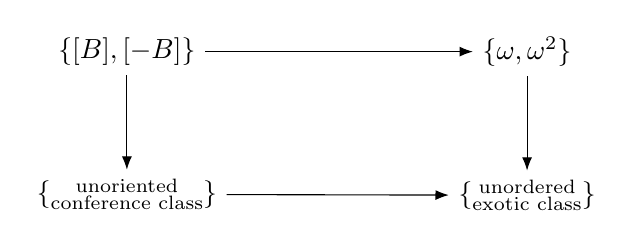
\begin{tikzpicture}[baseline=(current bounding box.center),
  node distance=12mm and 34mm,>=Latex]
\node (gold) {\(\{[B],[-B]\}\)};
\node[right=of gold] (field) {\(\{\omega,\omega^2\}\)};
\node[below=of gold] (ugold)
  {\(\{\substack{\text{unoriented}\\\text{conference class}}\}\)};
\node[below=of field] (ufield)
  {\(\{\substack{\text{unordered}\\\text{exotic class}}\}\)};
\draw[->] (gold) -- (field);
\draw[->] (gold) -- (ugold);
\draw[->] (field) -- (ufield);
\draw[->] (ugold) -- (ufield);
\end{tikzpicture}
\]
relative to the recovered six-set.
\end{theorem}

\begin{proof}
The equation \(\bar\varphi^2+\bar\varphi+1=0\) makes its restriction to the
simple heart primitive.  Reversal sends
\[
             B\longmapsto-B,\qquad
             \varphi\longmapsto1-\varphi,
\]
which reduces to \(\omega\mapsto1+\omega=\omega^2\).  The outer normalizer
exchanges the two \(G\)-invariant conference orientations and therefore acts
by the same involution.  Both vertical maps are principal \(C_2\)-torsors,
and the top map is equivariant and bijective, so the square is Cartesian.
\end{proof}

The lattice theorem and the modular extension theorem are classical in
nearby but separate forms: Chapman treats the skew/imaginary conference
analogue, while Bleher records the relevant uniserial block modules.  The
role of Theorem~\ref{thm:golden-frobenius} is their composition with the
orientation reconstructed in this paper.

\section{Residual Frobenius markings}
\label{sec:residual-markings}

Paper~IV ends with a different residual marking.  The comparison is governed
by the following standard descent lemma, not by a geometric arrow between
the papers.

\begin{lemma}[Frobenius-orbit commutant]
\label{lem:frobenius-orbit-commutant}
Let \(V\) be a simple \(\F_qG\)-module.  Suppose that after scalar extension
to an algebraic closure it is a multiplicity-free orbit
\[
               V_0\oplus V_0^{(q)}\oplus\cdots\oplus V_0^{(q^{r-1})}
\]
of \(r\) absolutely simple pairwise nonisomorphic constituents.  Then
\(\End_{\F_qG}(V)\cong\F_{q^r}\).  Selecting one constituent, equivalently
one embedding of this commutant field, is a principal
\(\Gal(\F_{q^r}/\F_q)\)-rigidification.
\end{lemma}

\begin{proof}
After scalar extension, Schur's lemma identifies the commutant with the
product of \(r\) scalar copies of the algebraic closure.  Frobenius permutes
the factors transitively.  Its fixed algebra is \(\F_{q^r}\), and its
embeddings are permuted simply transitively by the Galois group.
\end{proof}

For the upper branch, \(H_{\Omega_0}\) has commutant \(\F_4\); its two
constituents and the two primitive scalars form the \(C_2\)-torsor of
Theorem~\ref{thm:golden-frobenius}.  Paper~IV proves that its binary code is
simple, becomes a multiplicity-free Frobenius orbit of three
twelve-dimensional constituents, and has commutant \(\F_8\).  Its recovered
operators are
\[
                         \{\alpha,\alpha^2,\alpha^4\},
\]
a principal \(C_3\)-rigidification \cite{RuddPassant2026}.  The two examples
share the residual-field mechanism.  They have different groups, modules,
bases, and geometries, and no map between their carriers is asserted.

This completes the proof of Theorem~\ref{thm:normalization-residue-intro}
and explains the last arrow in the series map: Paper~V does not merge the
upper and lower branches; it identifies the common reason that their final
ambiguity is a Frobenius orbit.

\section{Verification and trust boundary}
\label{sec:verification}

Every load-bearing argument above is printed in the manuscript: the Hankel
Jacobian saturation, the stabilizer quotient, the outer-difference bridge,
the groupoid fibres, the root--weight saturation, and the triangle-presentation
Ext calculation.  The paper-owned standard-library checker
\begin{center}
\small\ttfamily
verification/evidence/paper\_ii\_chordal\_axis.py
\end{center}
has schema \texttt{paper-v-chordal-axis-v2}.  It independently reconstructs the matching
quotient from Paper II's frozen arithmetic, computes the central projector
and both intertwiner spaces, checks all cubic coefficients, enumerates the
rational singular loci, and determines the pencil action.  Its exact output
is the adjacent JSON file.  The JSON names, sizes, and hashes both frozen
inputs.  Their SHA-256 values
begin \texttt{d2100485} for the matching-module source and
\texttt{d45512c9} for the orbit-scout data; the unabbreviated values are part
of the machine-readable proof interface.  From the paper directory the
paper-local replay is
\begin{center}
\small\ttfamily
make evidence
\end{center}
and returns \texttt{CHECK OK (NO\_MATCH)}; \texttt{NO\_MATCH} records the
failure of the literal conference-line identification, not a failed check.
A separately written cold replay reproduced the normalized coefficient
vector; its full byte SHA-256 is recorded in the adjacent JSON certificate.
The execution is replay evidence for Proposition
\ref{prop:paper-ii-placement}, not a premise of the classification theorem.
In particular, it substitutes for none of Lemma
\ref{lem:hankel-singular-locus}, Proposition~\ref{prop:special-orbit},
Theorem~\ref{thm:conference-saturation}, or Proposition
\ref{prop:extension-line}.

\section{Conclusion}
\label{sec:conclusion}

The scattered shadows gather on one carrier, but not by becoming equal.
Paper~II supplies a chordal cubic; its special orbit returns the six axes;
outer difference returns the conference orientation of Papers~I and III.
The selected-line correspondence is an equivalence, and the bare
correspondence is exactly its \(C_2\)-quotient.  This is the complete
information-loss statement, including its scalar and outer sharpness.

The same six-set then separates two integral outputs that had previously
looked interchangeable.  The rank-five augmentation and rank-six
root--weight lattices meet only in their binary heart.  On the latter,
normalization before reduction converts the golden order into \(\F_4\), and
the residual geometric involution becomes Frobenius.  Paper~IV exhibits the
degree-three version of the same residual-field mechanism on an independent
carrier.  Thus the series ends not with a single universal model, but with a
structural answer to its recurring question: the missing marking is measured
by the commutant field of the shadow that survives.

\section*{AI assistance disclosure}

This project was developed with extensive assistance from OpenAI Codex and
Anthropic Claude. Under the author's direction, the systems assisted with
proof exploration, literature research, exact computation, verification,
and manuscript drafting and revision. The author checked the resulting
arguments, computations, code, and cited sources, reviewed and edited all
AI-assisted material, and assumes responsibility for all content.

\begin{thebibliography}{99}

\bibitem{BMS1979}
F.~C. Bussemaker, R.~A. Mathon, and J.~J. Seidel,
\newblock \emph{Tables of two-graphs},
\newblock EUT Report 79-WSK-05, Technische Hogeschool Eindhoven (1979),
doi:10.1007/BFb0092256.

\bibitem{Bleher2002}
F.~M. Bleher,
\newblock Universal deformation rings and Klein four defect groups,
\newblock \emph{Transactions of the American Mathematical Society}
\textbf{354} (2002), 3893--3906,
doi:10.1090/S0002-9947-02-03072-6.

\bibitem{Chapman2001}
R.~Chapman,
\newblock Conference matrices and unimodular lattices,
\newblock \emph{European Journal of Combinatorics} \textbf{22} (2001),
1033--1045, doi:10.1006/eujc.2001.0539.

\bibitem{CheltsovEtAl2025Chordal}
I.~Cheltsov, L.~Marquand, Y.~Tschinkel, and Z.~Zhang,
\newblock Equivariant geometry of cubic threefolds with non-isolated
singularities,
\newblock preprint (2025), arXiv:2505.03986.

\bibitem{GoethalsSeidel1967}
J.-M. Goethals and J.~J. Seidel,
\newblock Orthogonal matrices with zero diagonal,
\newblock \emph{Canadian Journal of Mathematics} \textbf{19} (1967),
1001--1010, doi:10.4153/CJM-1967-091-8.

\bibitem{HMSVOuter}
B.~Howard, J.~Millson, A.~Snowden, and R.~Vakil,
\newblock A description of the outer automorphism of \(S_6\), and the
invariants of six points in projective space,
\newblock \emph{Journal of Combinatorial Theory, Series A} \textbf{115}
(2008), 1296--1303, doi:10.1016/j.jcta.2008.01.004.

\bibitem{HaemersParsaeiMajd2022}
W.~H. Haemers and F.~Parsaei Majd,
\newblock Spectral symmetry in conference matrices,
\newblock \emph{Designs, Codes and Cryptography} \textbf{90} (2022),
1983--1990, doi:10.1007/s10623-021-00858-8.

\bibitem{PinardinZhang2025}
A.~Pinardin and Z.~Zhang,
\newblock \(A_5\)-equivariant geometry of quadric threefolds,
\newblock preprint (2025), arXiv:2508.11496v1.

\bibitem{RuddFactorization2026}
T.~Rudd,
\newblock Quadratic trade rigidity and cubic orientation in conic matching
quotients,
\newblock preprint (2026).

\bibitem{RuddRigidity2026}
T.~Rudd,
\newblock Reconstructing the Clebsch code and its golden orientation from its
deep-hole syndrome locus,
\newblock preprint (2026).

\bibitem{RuddPassages2026}
T.~Rudd,
\newblock Golden descent and operator realizations of the Clebsch cubic,
\newblock preprint (2026).

\bibitem{RuddPassant2026}
T.~Rudd,
\newblock Reconstructing \(\operatorname{PG}(2,13)\), its conic, and polarity
from the minimum words of a binary conic code,
\newblock preprint (2026).

\end{thebibliography}

\end{document}
